\documentclass[11pt, oneside]{article}   	% use "amsart" instead of "article" for AMSLaTeX format
\usepackage{geometry}                		% See geometry.pdf to learn the layout options. There are lots.
\usepackage{enumitem}
\usepackage{mathtools}

\geometry{letterpaper}                   		% ... or a4paper or a5paper or ... 
%\geometry{landscape}                		% Activate for rotated page geometry
%\usepackage[parfill]{parskip}    		% Activate to begin paragraphs with an empty line rather than an indent
\usepackage{graphicx}				% Use pdf, png, jpg, or eps§ with pdflatex; use eps in DVI mode
								% TeX will automatically convert eps --> pdf in pdflatex		
\usepackage{amssymb}
\usepackage{multicol}

\usepackage{xcolor}
\usepackage{textcomp}
\usepackage{subfigure}

%SetFonts

%SetFonts
% code listing settings
\usepackage{listings}
\lstset{
    language=Python,
    basicstyle=\ttfamily\small,
    aboveskip={1.0\baselineskip},
    belowskip={1.0\baselineskip},
    columns=fixed,
    extendedchars=true,
    breaklines=true,
    tabsize=4,
    prebreak=\raisebox{0ex}[0ex][0ex]{\ensuremath{\hookleftarrow}},
    frame=lines,
    showtabs=false,
    showspaces=false,
    showstringspaces=false,
    keywordstyle=\color[rgb]{0.627,0.126,0.941},
    commentstyle=\color[rgb]{0.133,0.545,0.133},
    stringstyle=\color[rgb]{01,0,0},
    numbers=left,
    numberstyle=\small,
    stepnumber=1,
    numbersep=10pt,
    captionpos=t,
    escapeinside={\%*}{*)}
}


\title{Project Report}
\author{Omar Ghaleb\\
COMP 5107}
\date{}							% Activate to display a given date or no date

\begin{document}
\renewcommand\thesubsection{\alph{subsection}.}
\maketitle
%\section{}
%\subsection{}
%\begin{enumerate}[label=\alph*)]
%	\item First item
%\end{enumerate}
\section*{Problem}
The idea of the project is to create a pattern classifier based on different methods and types of classifier on a selected dataset. In the project we created four main different classifiers:
\begin{itemize}
	\item Quadratic: Maximum Likelihood(ML), Bayesian(BL) and Parzen Window
	\item K-Nearest Neighbours
	\item Fisher's Discriminant 
	\item Ho-Kashyap
\end{itemize}
Each classifier was tested using five-cross validation.

\section*{Dataset}
The dataset selected is used to classify different types of glass. The reason for this is that identifying the type of glass helps in criminology. The data had no empty values thus it did not need to be cleaned. The data set contained 9 features(6 were selected) and two main classes and 9 subclasses. For our project we worked with the whole dataset as two main classes only which are (window or non-window). In the project, the data were projected on the first and second dimensions only (x1-x2).

The data was the normalized since the scales were far off from each other and affected the classification behaviour, hence, it was needed to make the scales similar by normalizing the data between 0 and 1. In Figure~\ref{fig:data-points}, we can see the effect of normalizing the data

\begin{figure}
\begin{center}
	\subfigure[Before Normalizing ]{
	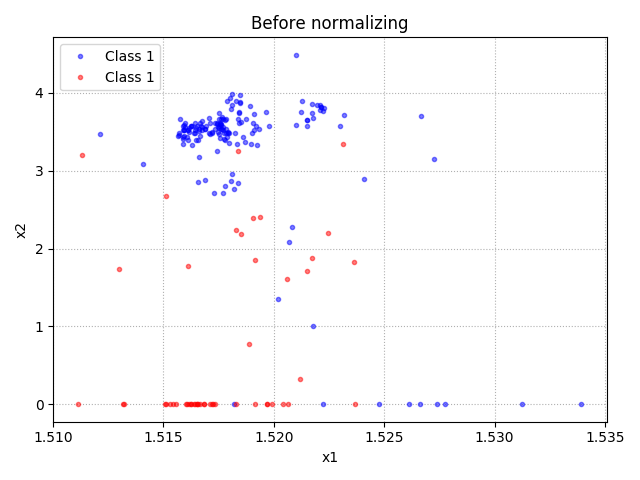
\includegraphics[width=0.45\textwidth]{plots/data-before-norm.png}
	\label{absorbing}
	}
	\subfigure[After Normalizing]{
	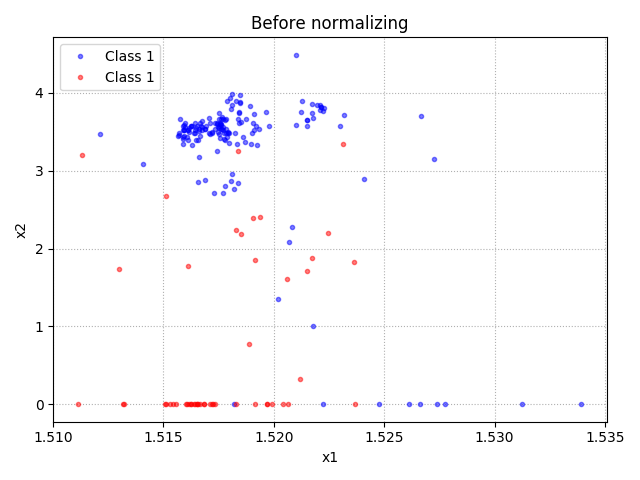
\includegraphics[width=0.45\textwidth]{plots/data-before-norm.png}
	\label{absorbing}
	}
\end{center}
\caption{Data Points in x1-x2 dimensions}
\label{fig:data-points}
\end{figure}

One problem with the data, and we will see the effect of that, is how close both classes are to each other as they both have very close means. Another problem is that the first class (window) consists of 3 times the instances of the other class(non-window).

\section*{Classifiers}
Below, we are going to go through our different classifiers that we created for this dataset.

\subsection{Quadratic Classifier}
First, we are going to talk about the quadratic classifiers (ML, BL, Parzen).
\subsubsection*{Maximum Likelihood (ML)}
\subsubsection*{Bayesian Learning (ML)}
\subsubsection*{Parzen Window}
\subsection{K-Nearest Neighbours Classifier}
\subsection{Fisher's Discriminant Classifier}
\subsection{Ho-Kashyap Classifier}
%In this assignment we have two classes $X_1$ and $X_2$ with means same as the previous assignments $M_1$ and $M_2$ where: $$M_1 = \begin{bmatrix}
%3 & 1 & 4 
%\end{bmatrix},\quad M_2 = \begin{bmatrix}
%-3 & 1 & -4 
%\end{bmatrix}$$
%  and covariance matrices as follows: 
%  $$\Sigma_{X_1} = \begin{bmatrix}
%a^2 & \beta ab & \alpha ac \\
%\beta ab & b^2 & \beta bc \\
%\alpha ac & \beta bc & c^2 
%\end{bmatrix},\quad \Sigma_{X_2} = \begin{bmatrix}
%c^2 & \alpha bc & \beta ac \\
%\alpha bc & b^2 & \alpha ab \\
%\beta ac & \alpha ab & a^2 
%\end{bmatrix}$$
%
%The parameters used in this assignment is as follows:
%$$ a=2,\quad b=3,\quad c=4,\quad \alpha=0.1,\quad \beta=0.2,\quad \#points = 200 $$
%This resulted the covariance matrices to have the following values:
%$$\Sigma_{X_1} = \begin{bmatrix}
%4 & 1.2 & 0.8 \\
%1.2 & 9 & 2.4 \\
%0.8 & 2.4 & 16 
%\end{bmatrix}, \quad \Sigma_{X_2} = \begin{bmatrix}
%16 & 1.2 & 1.6 \\
%1.2 & 9 & 0.6 \\
%1.6 & 0.6 & 4 
%\end{bmatrix}$$


%%%%%%%%%%%%%%%%%%%%%%%%%%%%%%%%%%%%%%%%%%%%%%%%%%%%%%%%%%%%%%%%
\subsection{Create points for each distribution:}

Here we used the same exact methods for creating the points from the previous assignment.
And the plots of the points are available below.

\begin{lstlisting}[label={list:first},caption=points generation]
# create point matrices for the two classes X1 and X2
z1_training_points, x1_training_points = h.generate_point_matrix(v_x1, lambda_x1, m1, number_of_points)
z2_training_points, x2_training_points = h.generate_point_matrix(v_x2, lambda_x2, m2, number_of_points)
\end{lstlisting}



%%%%%%%%%%%%%%%%%%%%%%%%%%%%%%%%%%%%%%%%%%%%%%%%%%%%%%%%%%%%%%%%
\subsection{Estimate the ML and BL:}

To estimate the parameters for both data sets using ML:
$$ \hat{M}=\frac{1}{N} \sum_{i=1}^{N} x_i, \quad\quad \hat{\Sigma}=	 frac{1}{N} \sum_{i=1}^{N}[X_i-\hat{M}][X_i-\hat{M}]^T$$


\begin{lstlisting} [label={list:first},caption=ML and BL mean and covariance]
def estimate_mean_ml(points, n):
    points = np.array(points)
    points = points[:, :n]
    mean = np.sum(points, axis=1)
    mean = mean / n
    mean = np.array(mean)[np.newaxis]
    return mean.transpose()

def estimate_cov_ml(points, mean, n):
    points = np.array(points)
    mean = np.array(mean)
    cov = (points - mean) @ (points - mean).transpose()
    cov = cov / n
    return cov

def estimate_mean_bl(points, mean0, cov_initial, cov_actual, n):
    points = np.array(points)
    points = points[:, :n]
    mean0 = np.array(mean0)
    cov_initial = np.array(cov_initial)
    cov_actual = np.array(cov_actual)
    points_sum = np.sum(points, axis=1) / n
    points_sum = np.array(points_sum)[np.newaxis]
    points_sum = points_sum.transpose()

    m = cov_actual / n @ np.linalg.inv(
        cov_actual / n + cov_initial) @ mean0 + cov_initial @ np.linalg.inv(
        cov_actual / n + cov_initial) @ points_sum
    return m
\end{lstlisting}

And these were the results of ML:$$\hat{M_1} = \begin{bmatrix}
3.22 \\ 1.23 \\ 4.16 
\end{bmatrix},\quad \hat{M_2} = \begin{bmatrix}
-2.85 \\ 1.23 \\ -4.09 
\end{bmatrix}$$
$$\hat{\sum_{X_1}} = \begin{bmatrix}
4.30 & 1.22 & 1.29 \\
1.22 & 9.81 & 2.35 \\
1.29 & 2.35 & 14.49 
\end{bmatrix}, \quad \hat{\sum_{X_2}} = \begin{bmatrix}
17.75 & 0.97 & 2.57 \\
0.97 & 8.48 & 1.21 \\
2.57 & 1.21 & 4.13 
\end{bmatrix}$$\\


Then we used BL to estimate the mean is using the following equation:
$$\left(m\right)_n=\frac{1}{n}\Sigma\left[\frac{1}{n}\Sigma+\Sigma_0\right]^{-1}m_0+\Sigma_0\left[\frac{1}{n}\Sigma+\Sigma_0\right]^{-1}\left(\frac{1}{n}\sum_{j=1}^{n}x_j\right)$$

The resulting means are as below:
$$\hat{M_1} = \begin{bmatrix}
3.22 \\ 1.24 \\ 4.13 
\end{bmatrix},\quad \hat{M_2} = \begin{bmatrix}
-2.85 \\ 1.23 \\ -4.10 
\end{bmatrix}$$

\begin{figure}
\begin{center}
	\subfigure[ML Mean]{
	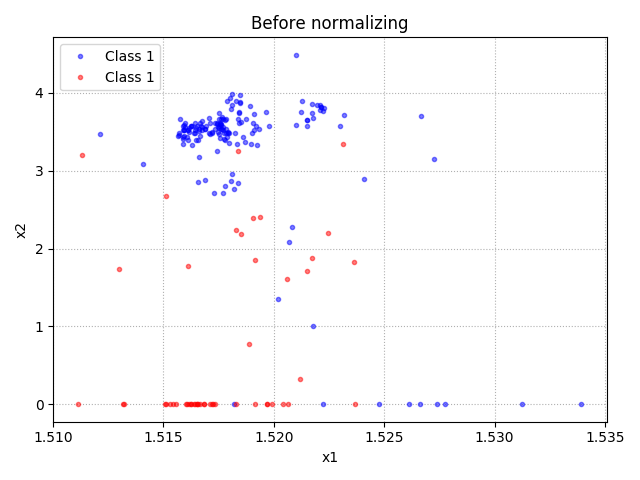
\includegraphics[width=0.45\textwidth]{plots/data-before-norm.png}
	\label{absorbing}
	}
	\subfigure[ML Covariance]{
	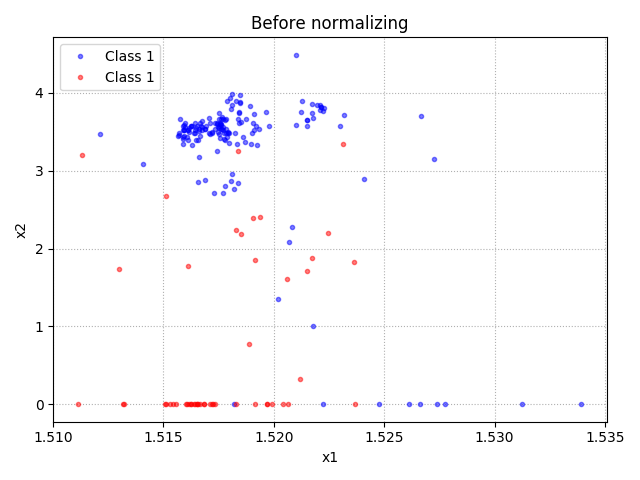
\includegraphics[width=0.45\textwidth]{plots/data-before-norm.png}
	\label{absorbing}
	}\\
	\subfigure[BL Mean]{
	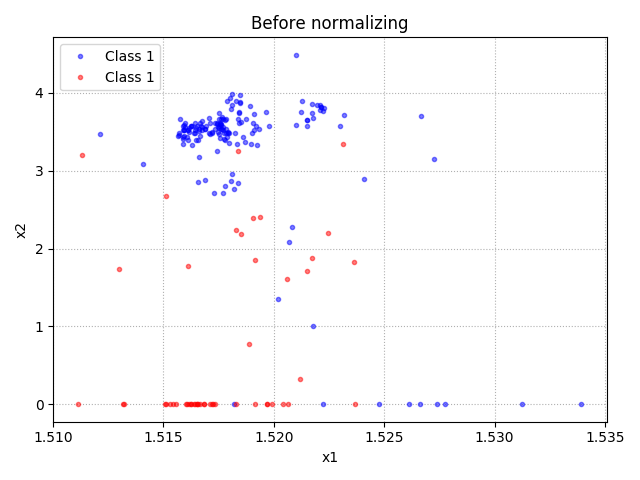
\includegraphics[width=0.45\textwidth]{plots/data-before-norm.png}
	\label{absorbing}
	}
\end{center}
\caption{Mean and covariance Convergances}
\end{figure}

%%%%%%%%%%%%%%%%%%%%%%%%%%%%%%%%%%%%%%%%%%%%%%%%%%%%%%%%%%%%%%%%
\subsection{Use Parzen window approach:}
In this part we are going to use Parzen window, gaussian kernels, to estimate the means and density functions of each dimension. The kernel function used is:
$$\hat{f_i}(x)=\frac{1}{N}\sum_{i=1}^{N}\frac{1}{\sqrt{2\pi}\sigma} e^{-\frac{(x-x_i)^2}{2\sigma^2}} $$

The estimated mean:
$$\hat{m}=\sum_{x}x\hat{f}(x)\Delta x $$

The estimated covariance:
$$\hat{\sigma}^2=\sum_{x}(x-\hat{m})^2\hat{f}(x)\Delta x$$

\begin{lstlisting} [label={list:first},caption=Parzen window Code]
def kernel_function(x, xi, cov):
    result = (1 / (math.sqrt(2 * math.pi) * cov)) * math.exp(-math.pow(x - xi, 2) / (2 * math.pow(cov, 2)))
    return result

def parzen_expected_mean(x, f_x, delta_x):
    return x * f_x * delta_x

def parzen_expected_covariance(x, f_x, delta_x, mean):
    return math.pow(x - mean, 2) * f_x * delta_x
\end{lstlisting}

And these were the results of Parzen:$$\hat{M_1} = \begin{bmatrix}
3.19 \\ 1.21 \\ 4.12 
\end{bmatrix},\quad \hat{M_2} = \begin{bmatrix}
-2.87 \\ 1.20 \\ -4.09 
\end{bmatrix}$$
$$\hat{\sum_{X_1}} = \begin{bmatrix}
4.28 & 0 & 0 \\
0 & 9.69 & 0 \\
0 & 0 & 14.32 
\end{bmatrix}, \quad \hat{\sum_{X_2}} = \begin{bmatrix}
17.51 & 0 & 0 \\
0 & 8.33 & 0 \\
0 & 0 & 4.09 
\end{bmatrix}$$\\


\begin{figure}
\begin{center}
	\subfigure[$x_1$ estimated $\hat{f}(x)$]{
	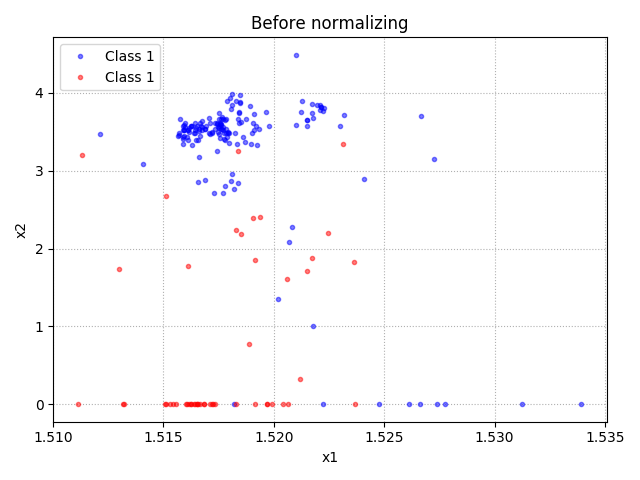
\includegraphics[width=0.45\textwidth]{plots/data-before-norm.png}
	\label{absorbing}
	}
	\subfigure[$x_2$ estimated $\hat{f}(x)$]{
	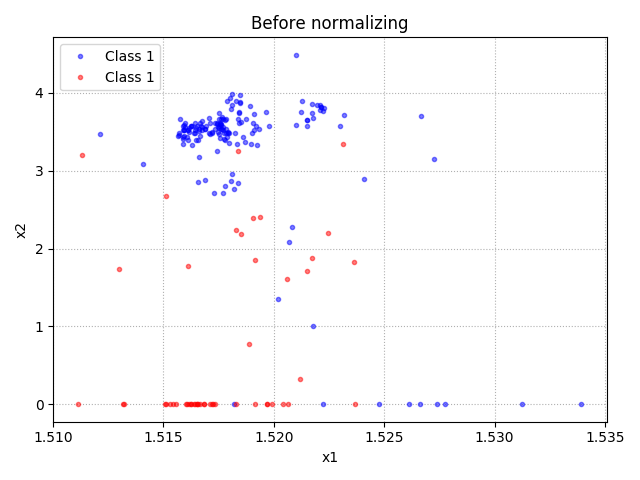
\includegraphics[width=0.45\textwidth]{plots/data-before-norm.png}
	\label{absorbing}
	}\\
	\subfigure[$x_3$ estimated $\hat{f}(x)$]{
	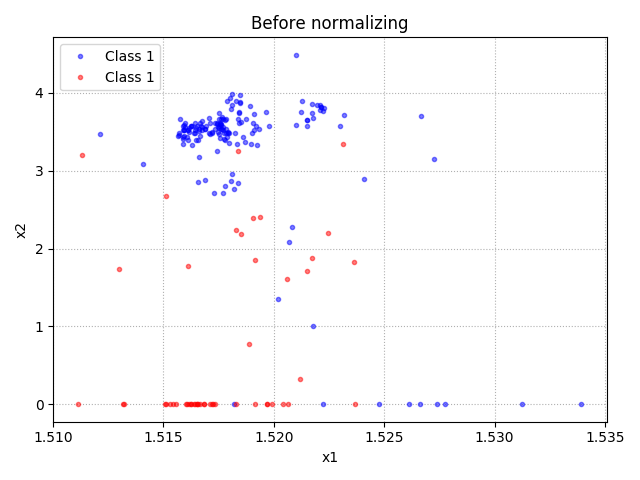
\includegraphics[width=0.45\textwidth]{plots/data-before-norm.png}
	\label{absorbing}
	}
\end{center}
\caption{Density Functions Estimation using Parzen Window}
\end{figure}


%%%%%%%%%%%%%%%%%%%%%%%%%%%%%%%%%%%%%%%%%%%%%%%%%%%%%%%%%%%%%%%%

\subsection{Compute Bayes discriminant function for ML, BL and Parzen:}
Here I used the same code from the previous assignment to calculate the discriminant function for the three methods. And the results are in the figure below.

\begin{figure}
\begin{center}
	\subfigure[$x_1$ estimated $\hat{f}(x)$]{
	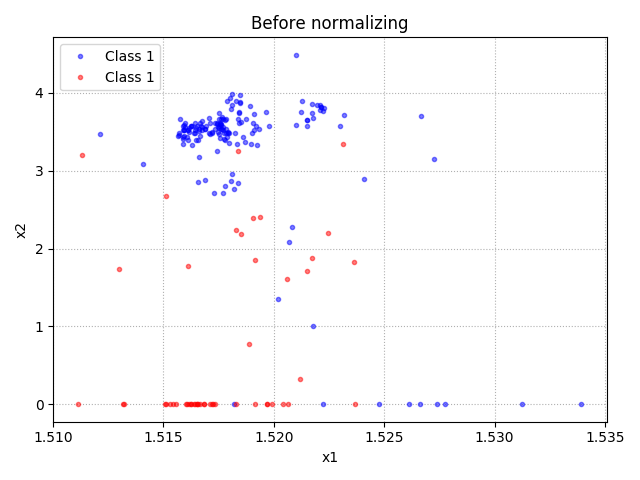
\includegraphics[width=0.45\textwidth]{plots/data-before-norm.png}
	\label{absorbing}
	}
	\subfigure[$x_2$ estimated $\hat{f}(x)$]{
	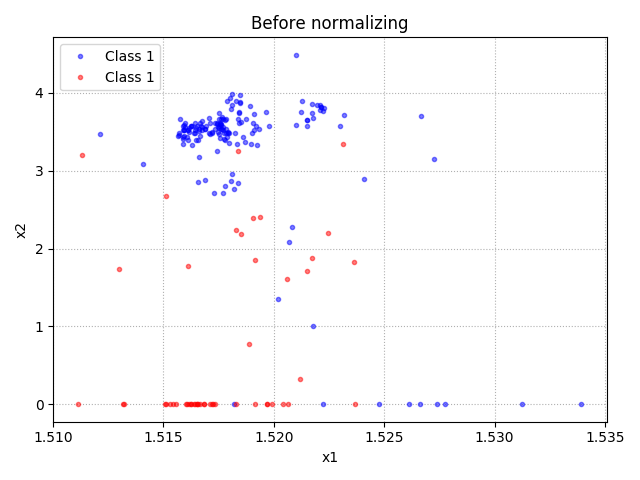
\includegraphics[width=0.45\textwidth]{plots/data-before-norm.png}
	\label{absorbing}
	}\\
	\subfigure[$x_3$ estimated $\hat{f}(x)$]{
	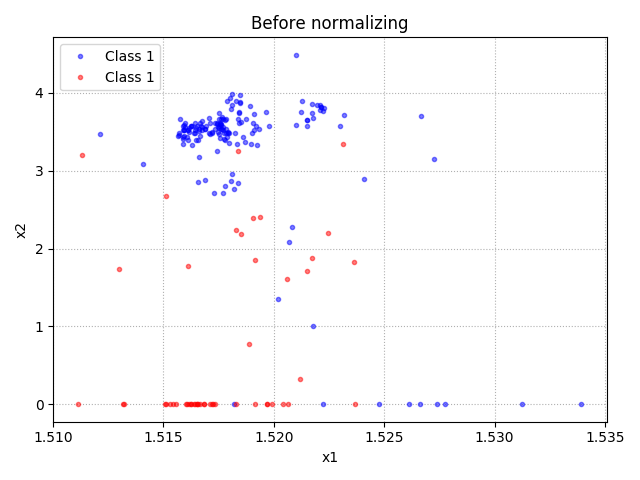
\includegraphics[width=0.45\textwidth]{plots/data-before-norm.png}
	\label{absorbing}
	}
	\subfigure[$x_1$ estimated $\hat{f}(x)$]{
	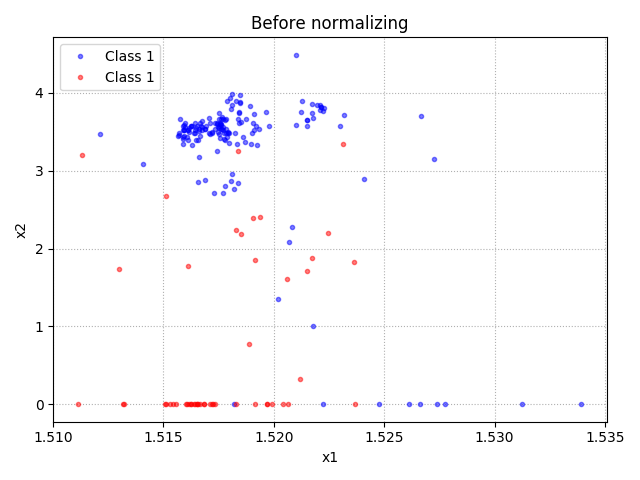
\includegraphics[width=0.45\textwidth]{plots/data-before-norm.png}
	\label{absorbing}
	}\\
	\subfigure[$x_2$ estimated $\hat{f}(x)$]{
	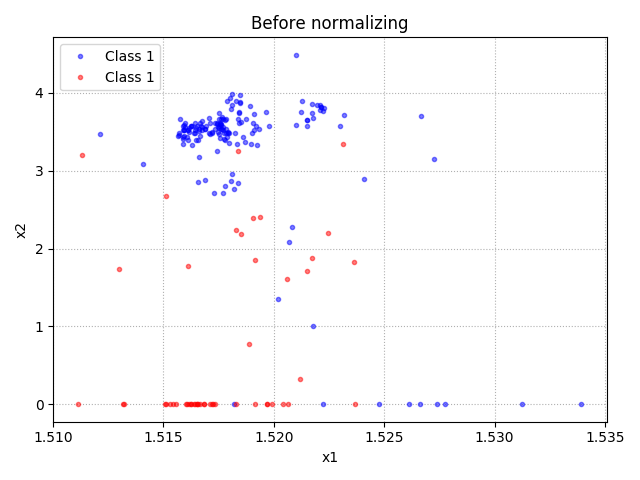
\includegraphics[width=0.45\textwidth]{plots/data-before-norm.png}
	\label{absorbing}
	}
	\subfigure[$x_3$ estimated $\hat{f}(x)$]{
	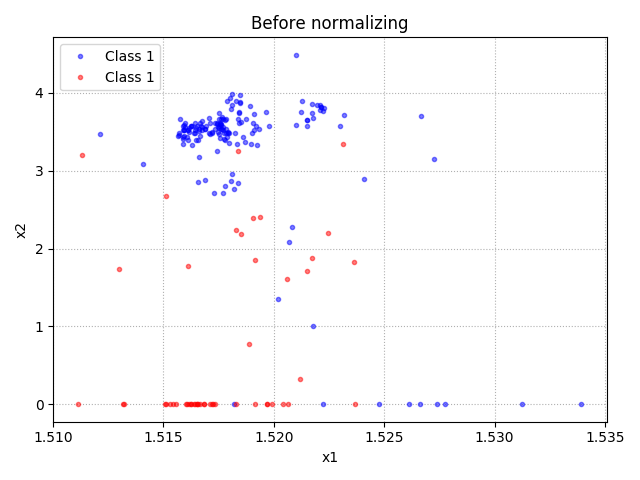
\includegraphics[width=0.45\textwidth]{plots/data-before-norm.png}
	\label{absorbing}
	}
\end{center}
\caption{Density Functions Estimation using Parzen Window}
\end{figure}

%%%%%%%%%%%%%%%%%%%%%%%%%%%%%%%%%%%%%%%%%%%%%%%%%%%%%%%%%%%%%%%%

\subsection{Use 10-Cross validation to test the classifiers:}
We created 200 more points for each class so we have 400 points total for each class.\\

\begin{lstlisting} [label={list:first},caption=K-cross validation]
test_results_ml_class1 = []
test_results_ml_class2 = []

test_results_bl_class1 = []
test_results_bl_class2 = []

test_results_parzen_class1 = []
test_results_parzen_class2 = []

k = 10

class1_total_points = v1_training_points
class1_total_points = np.append(class1_total_points, v1_test_points, axis=1)

class2_total_points = v2_training_points
class2_total_points = np.append(class2_total_points, v2_test_points, axis=1)

print(class1_total_points[:, 399])
n = number_of_points + test_points_count
for i in range(0, k, 1):
    print('Cross:' + str(i+1))
    number_of_testing_points = int(n / k)
    number_of_training_points = int(n - n / k)
    start = int(n * i / k)
    end = int((i + 1) * n / k - 1)

    class1_test_points = class1_total_points[:, start: end]
    class1_train_points = class1_total_points[:, 0:start]
    class1_train_points = np.append(class1_train_points, class1_total_points[:, end:], axis=1)

    class2_test_points = class2_total_points[:, start: end]
    class2_train_points = class2_total_points[:, 0:start]
    class2_train_points = np.append(class2_train_points, class2_total_points[:, end:], axis=1)

    # estimated mean using ML
    x1_ml_estimated_mean = h.estimate_mean_ml(class1_train_points, number_of_training_points)
    x1_ml_estimated_cov = h.estimate_cov_ml(class1_train_points, x1_ml_estimated_mean, number_of_training_points)

    x2_ml_estimated_mean = h.estimate_mean_ml(class2_train_points, number_of_points)
    x2_ml_estimated_cov = h.estimate_cov_ml(class2_train_points, x2_ml_estimated_mean, number_of_training_points)

    # Estimating the means using BL
    x1_bl_estimated_mean, x2_bl_estimated_mean = h.bl_expected_mean(class1_train_points, class2_train_points, sigma_v1, sigma_v2, v1_mean, v2_mean, number_of_training_points)

    # estimated mean and cov using parzen window
    x1_parzen_estimated_mean, x1_parzen_estimated_covariance, x2_parzen_estimated_mean, x2_parzen_estimated_covariance = h.estimated_mean_parzen(class1_train_points, class2_train_points, kernel_covariance, step_size)

    ml_class1_accuracy, ml_class2_accuracy = h.test_classifier(class1_test_points, class2_test_points, x1_ml_estimated_cov, x2_ml_estimated_cov, x1_ml_estimated_mean, x2_ml_estimated_mean, number_of_testing_points)
    test_results_ml_class1 = np.append(test_results_ml_class1, ml_class1_accuracy)
    test_results_ml_class2 = np.append(test_results_ml_class2, ml_class2_accuracy)

    bl_class1_accuracy, bl_class2_accuracy = h.test_classifier(class1_test_points, class2_test_points, sigma_v1, sigma_v2, x1_bl_estimated_mean, x2_bl_estimated_mean, number_of_testing_points)
    test_results_bl_class1 = np.append(test_results_bl_class1, bl_class1_accuracy)
    test_results_bl_class2 = np.append(test_results_bl_class2, bl_class2_accuracy)

    parzen_class1_accuracy, parzen_class2_accuracy = h.test_classifier(class1_test_points, class2_test_points, x1_parzen_estimated_covariance, x2_parzen_estimated_covariance, x1_parzen_estimated_mean, x2_parzen_estimated_mean, number_of_testing_points)
    test_results_parzen_class1 = np.append(test_results_parzen_class1, parzen_class1_accuracy)
    test_results_parzen_class2 = np.append(test_results_parzen_class2, parzen_class2_accuracy)
\end{lstlisting}

And the resulting testing accuracy is as follows:
\begin{lstlisting} [label={list:first},caption=Accuracy before Diagonalization]
ML Accuracy before Diagonalization:
+---------+----------+
|         | Accuracy |
+---------+----------+
| class 1 |  88.75   |
| class 2 |  93.75   |
+---------+----------+

BL Accuracy before Diagonalization:
+---------+----------+
|         | Accuracy |
+---------+----------+
| class 1 |   89.5   |
| class 2 |  94.25   |
+---------+----------+

Parzen Accuracy before Diagonalization:
+---------+----------+
|         | Accuracy |
+---------+----------+
| class 1 |  91.75   |
| class 2 |   90.5   |
+---------+----------+

\end{lstlisting}

%%%%%%%%%%%%%%%%%%%%%%%%%%%%%%%%
\break
\subsection{Diagonalize the points and redo everything:}
After diagonalizing the data, I will only include the results obtained using the same methods.

%\begin{figure}
%\begin{center}
%	\subfigure[v1-v2]{
%	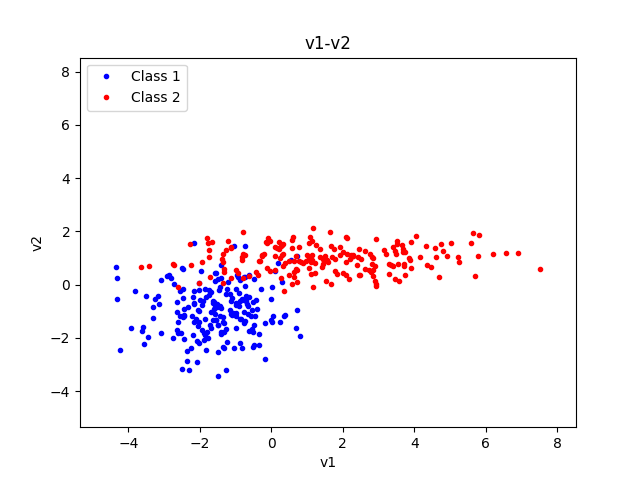
\includegraphics[width=0.45\textwidth]{v1-v2-points.png}
%	\label{absorbing}
%	}
%	\subfigure[v1-v3]{
%	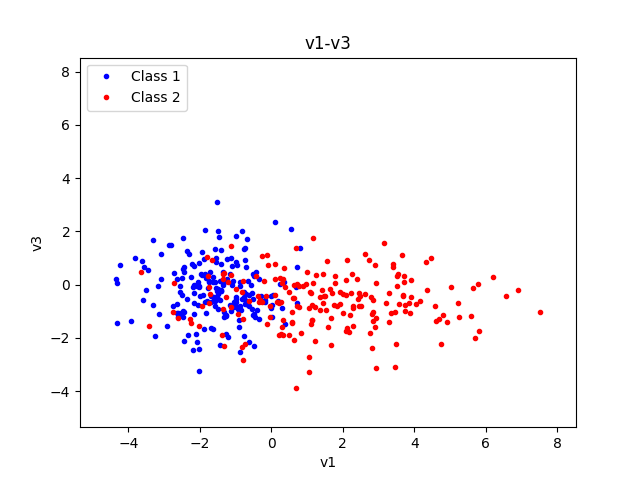
\includegraphics[width=0.45\textwidth]{v1-v3-points.png}
%	\label{absorbing}
%	}
%\end{center}
%\caption{Training points after diagonalization}
%\end{figure}
%
%\begin{figure}
%\begin{center}
%	\subfigure[ML Mean]{
%	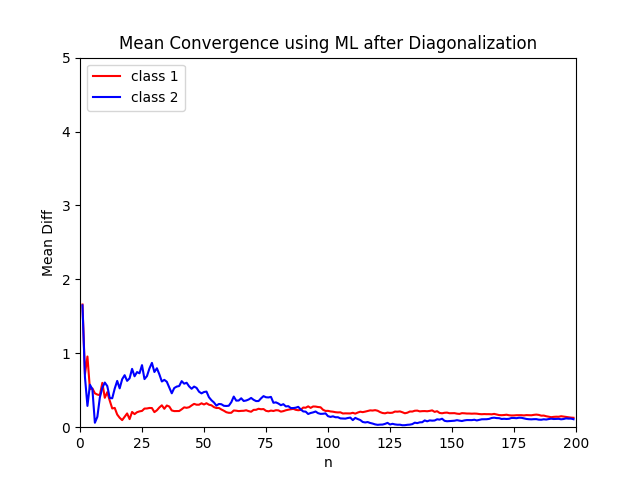
\includegraphics[width=0.45\textwidth]{ML-mean-convergance-after.png}
%	\label{absorbing}
%	}
%	\subfigure[ML Covariance]{
%	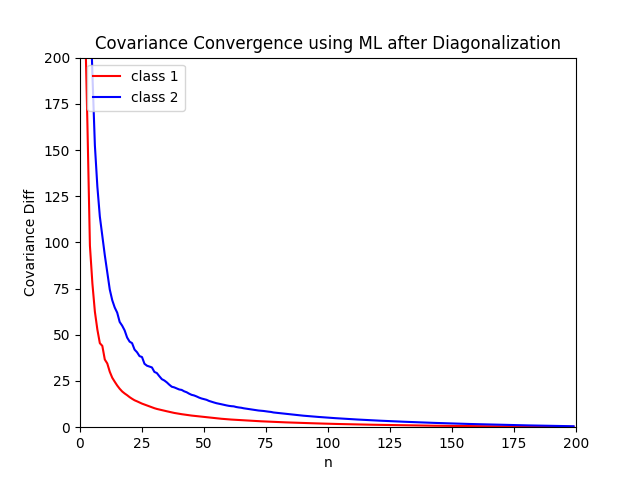
\includegraphics[width=0.45\textwidth]{ML-cov-convergance-after.png}
%	\label{absorbing}
%	}\\
%	\subfigure[BL Mean]{
%	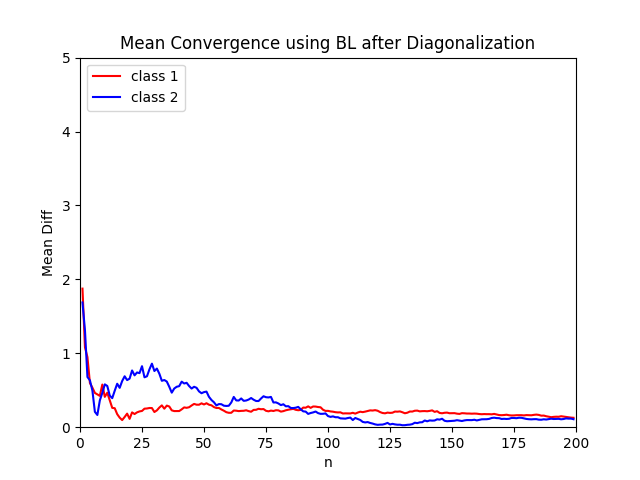
\includegraphics[width=0.45\textwidth]{BL-mean-convergance-after.png}
%	\label{absorbing}
%	}
%\end{center}
%\caption{Mean and covariance Convergances after diagonalization}
%\end{figure}
%
%\begin{figure}
%\begin{center}
%	\subfigure[$x_1$ estimated $\hat{f}(x)$]{
%	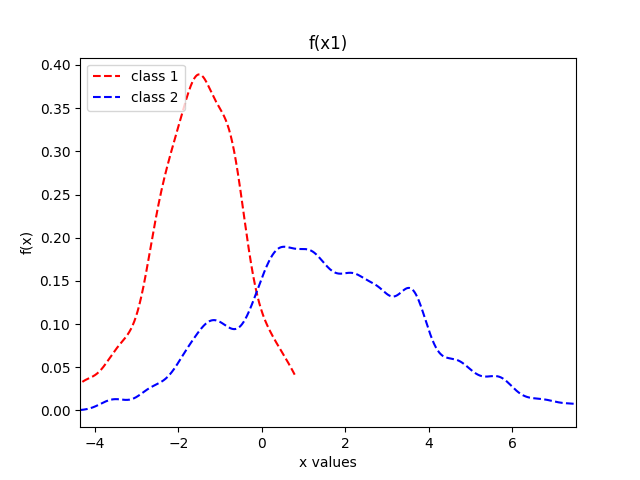
\includegraphics[width=0.45\textwidth]{x1-density-estimation-parzen-after.png}
%	\label{absorbing}
%	}
%	\subfigure[$x_2$ estimated $\hat{f}(x)$]{
%	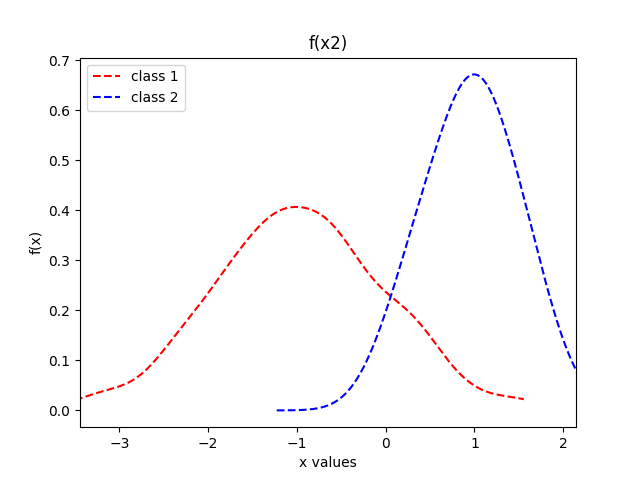
\includegraphics[width=0.45\textwidth]{x2-density-estimation-parzen-after.png}
%	\label{absorbing}
%	}\\
%	\subfigure[$x_3$ estimated $\hat{f}(x)$]{
%	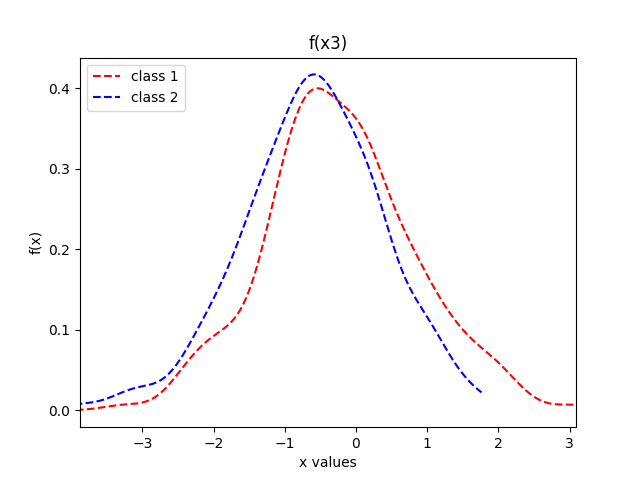
\includegraphics[width=0.45\textwidth]{x3-density-estimation-parzen-after.png}
%	\label{absorbing}
%	}
%\end{center}
%\caption{Density Functions Estimation using Parzen Window after diagonalization}
%\end{figure}
%
%\begin{figure}
%\begin{center}
%	\subfigure[$x_1$ estimated $\hat{f}(x)$]{
%	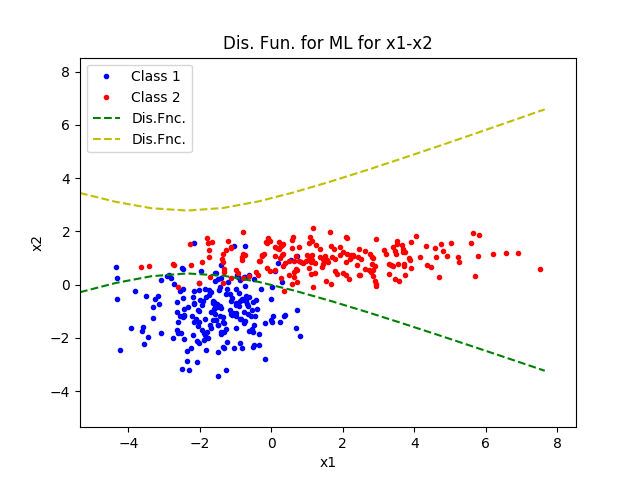
\includegraphics[width=0.45\textwidth]{x1-x2-Disc-func-ML-after.png}
%	\label{absorbing}
%	}
%	\subfigure[$x_2$ estimated $\hat{f}(x)$]{
%	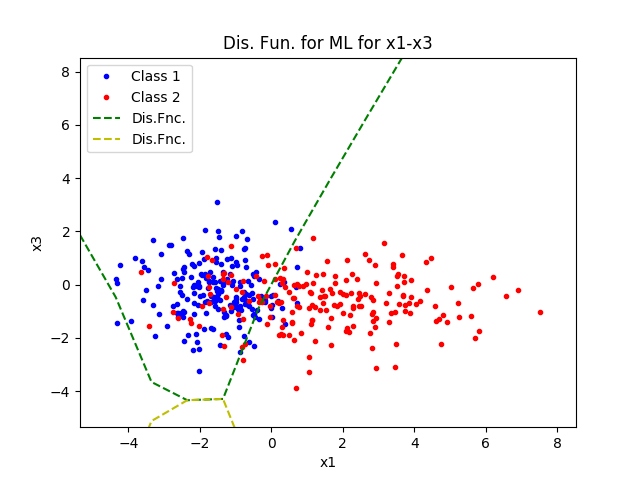
\includegraphics[width=0.45\textwidth]{x1-x3-Disc-func-ML-after.png}
%	\label{absorbing}
%	}\\
%	\subfigure[$x_3$ estimated $\hat{f}(x)$]{
%	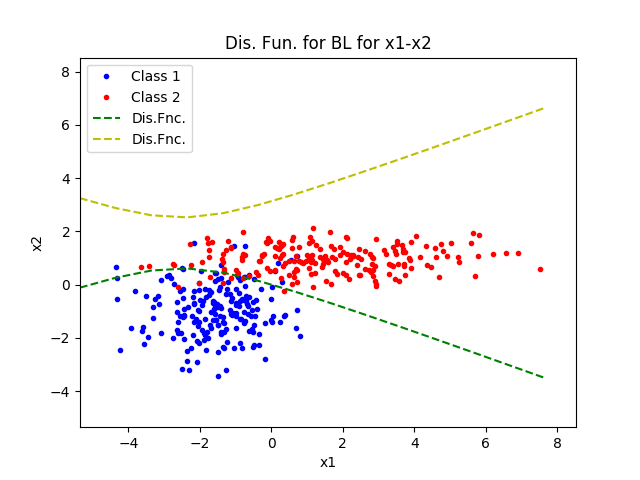
\includegraphics[width=0.45\textwidth]{x1-x2-Disc-func-BL-after.png}
%	\label{absorbing}
%	}
%	\subfigure[$x_1$ estimated $\hat{f}(x)$]{
%	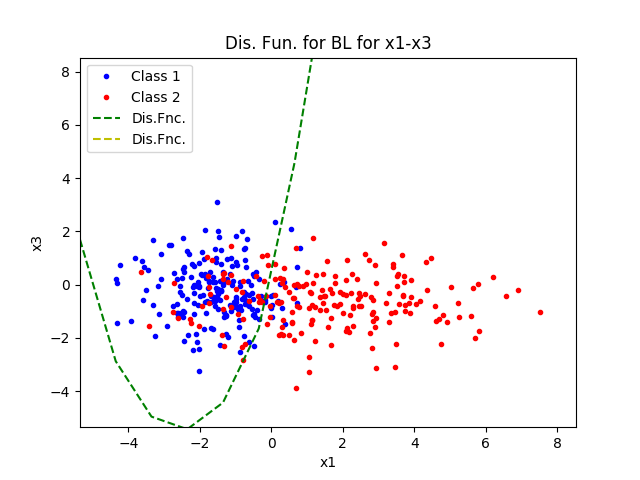
\includegraphics[width=0.45\textwidth]{x1-x3-Disc-func-BL-after.png}
%	\label{absorbing}
%	}\\
%	\subfigure[$x_2$ estimated $\hat{f}(x)$]{
%	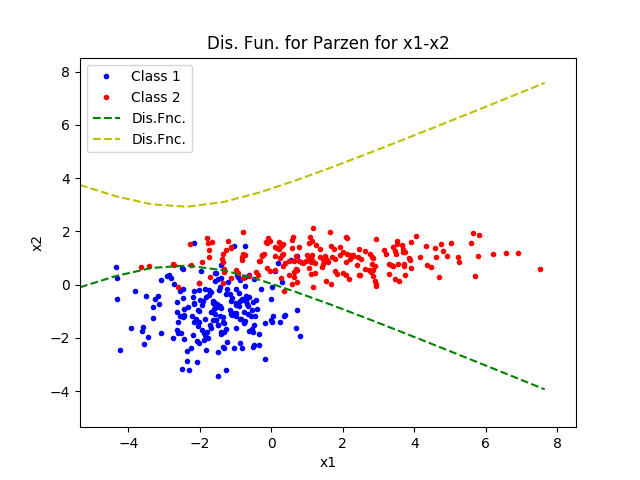
\includegraphics[width=0.45\textwidth]{x1-x2-Disc-func-parzen-after.png}
%	\label{absorbing}
%	}
%	\subfigure[$x_3$ estimated $\hat{f}(x)$]{
%	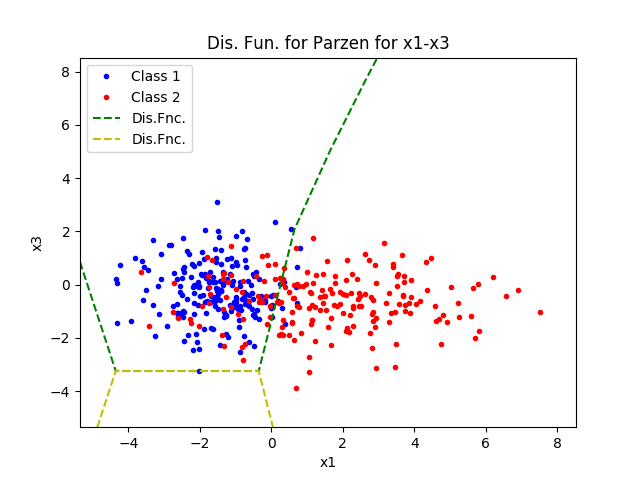
\includegraphics[width=0.45\textwidth]{x1-x3-Disc-func-parzen-after.png}
%	\label{absorbing}
%	}
%\end{center}
%\caption{Discriminant Functions after diagonalization}
%\end{figure}
%\break
%And the resulting testing accuracy is as follows:
%\begin{lstlisting} [label={list:first},caption=Accuracy after Diagonalization]
%ML Accuracy After Diagonalization:
%+---------+----------+
%|         | Accuracy |
%+---------+----------+
%| class 1 |  88.75   |
%| class 2 |  93.75   |
%+---------+----------+
%
%BL Accuracy after Diagonalization:
%+---------+----------+
%|         | Accuracy |
%+---------+----------+
%| class 1 |   89.5   |
%| class 2 |   94.5   |
%+---------+----------+
%
%Parzen Accuracy after Diagonalization:
%+---------+----------+
%|         | Accuracy |
%+---------+----------+
%| class 1 |   91.5   |
%| class 2 |  92.25   |
%+---------+----------+
%
%\end{lstlisting}

\end{document}  








